\section{Introduction}

\subsection{Theory}

Resistance can be measured using two methods: direct or indirect. To take a direct measurement, the measured component must be connected to the ohmmeter as shown in Fig.~\ref{fig:direct_schematic}. The component cannot be connected to a circuit, and must be passive and linear. The final result is obtained by calculating the limiting error and applying it to the measured value.

\begin{figure}[H]
	\centering
	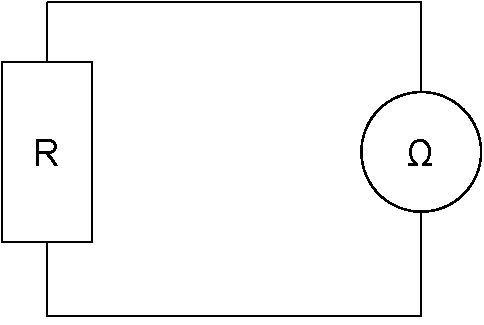
\includegraphics[width=6cm]{schematics/direct.pdf}
	\caption{Direct resistance measurement schematic}
	\label{fig:direct_schematic}
\end{figure}

\subsection{Equipment}

The following devices were used during the laboratory:

\begin{itemize}
	\item digital meter: UT803;
	\item linear resistor;
	\item diode resistor.
\end{itemize}